
\chapter{Analýza} \label{analyza}

\section{Architektura řešení} \label{architektura_reseni}

<DIAGRAM with protocols>

Parkovací systém se zkládá z následujících částí, které si nyní popíšeme stručně a detailněji později:

\begin{itemize}
  \item \textbf{Backend} je středobodem celé aplikace -- komunikuje se všemy ostatními komponentami.
        Zajišťuje business logiku aplikace, autentizaci i autorizaci uživatelů a perzistenci dat do \textbf{Databáze}.
  \begin{itemize}
    \item \textbf{Databáze} (nevlastní software -- https://www.mongodb.com/) k ukládání dat je MongoDB, která byla vybrána, protože data se budou
          převážně zapisovat a bude potřeba v nich rychle hledat a provádět agregační dotazy.
    \item \textbf{OpenALPR Server} (převzato z https://github.com/gerhardsletten/express-openalpr-server) je server, jenž obstarává přístup
          ke knihovně OpenALPR (https://github.com/openalpr/openalpr), která rozpoznává SPZ, přes protokol http.
  \end{itemize}
  \item \textbf{Mobilní aplikace} posílá obrazová data na \textbf{Backend}, kde jsou zpracována. Je určena pro platformu Android.
  \item \textbf{Frontend} je rozhraní mezi celým systémem a správcem parkoviště a dalšího personálu.
\end{itemize}

% - describe all superficially
% - in their subsections, be specific

\section{Volba technologií a vývojového prostředí} \label{devenv}

Jako programovací jazyk pro \textbf{Backend} byl zvolen staticky typovaný Typescript kvůli rychlosti vývoje
a množství knihoven, které poskytuje ekosystém Node.js. Primárním způsobem komunikace s \textbf{Frontend}
je dotazovací jazyk GraphQL, který přináší ucelený popis poskytovanách dat pomocí kontroly typů,
expresivních dotazů, jejichž odpověď má stejný "tvar". Obrázek \ref{fig:graphql_example} ukazuje dotaz hledání uživatele podle jména.

\begin{figure} \centering
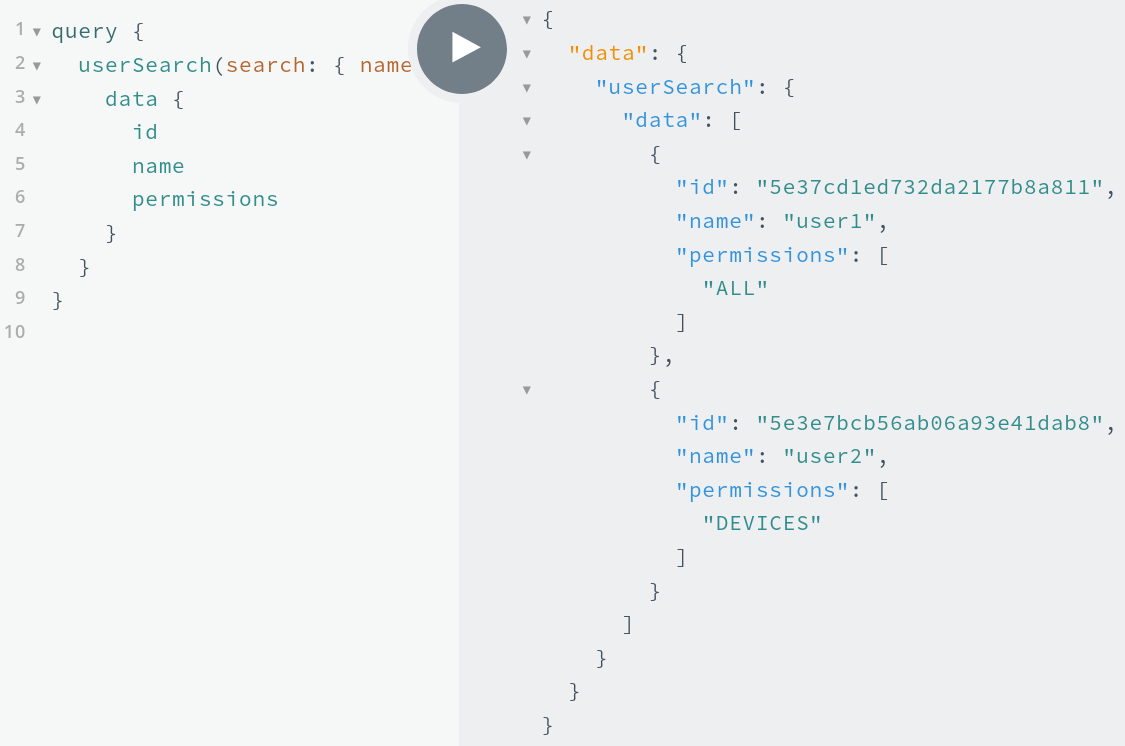
\includegraphics[width=145mm]{../img/graphql_example.png}
\caption{Screenshot z nástroje GraphQL Playground. Příklad GraphQL dotazu (vlevo) a odpovědi (vpravo).}
\label{fig:graphql_example}
\end{figure}

Model uživatele může mít i další atributy, ale GraphQL vrátí přesně ty údaje, na které se uživatel zeptal.
Tento triviální příklad neukazuje další funkce jako argumenty, mutace dat, dědičnost, více dotazů v jednom http dotazu
a mnoho dalších.
GraphQL je pouze specifikace vytvořená společností Facebook. Detailní informace jsou dostupné na oficiálních
stránkach https://graphql.org/.

Pro \textbf{Frontend} byl jako u \textbf{Backend} vybrán Typescript ze stejných důvodů. Renderování zajišťuje
knihovna React, která od řekněme klasického přístupu, kdy se odděluje HTML a Javascript do separátních
souborů, mandatuje, že v jednom souboru je jedna komponenta se vším svým HTML a logikou ve formě Javascriptu nebo
Typescriptu. Pomocí knihovny typestyle pak můžeme do stejného souboru psát i typované CSS.
Aby bylo možné snadno sdílet mezi komponentami stav, byla pro takzvaný state-management zvolena knihovna Redux.

\textbf{Mobilní aplikace}, která je určena pro platformu Android, měla volbu jazyka omezenou na Javu, Kotlin a C++.
Rychlost C++ není potřeba a navíc autor s tímto jazykem nižší úrovně nemá takové zkušenosti.
Kotlin oproti Javě umožňuje přímočarejší přístup k elementům uživatelského rozhraní, a proto byl zvolen.

% Maybe divide into smaller pieces

% Typescript
% - rychlost vývoje JS
% - type safety
% - Node ecosystem
%   - dev tools
%   - libraries
%   - npm
% - freedom of expression
% - scripts using main code

% VSCode
% - supports TS well
% - lightweight
% - plethora of extensions to ease development

% Docker for deployment

% TODO: Find a better label
\subsection{Detekce SPZ}

% - just a phone taking photographs and analyzing them
%   - in the phone (rooted and/or with a normal Linux distro)
%   - remotely through back end
% - movement detection
% - size to filter distant vehicles that are not entering etc.

\subsection{Serverová aplikace}

% - Express
%   - standard and other libraries build on it
%   - REST for Devices
% - JEST \& Supertest
%   - declarative simple
%   - integrates with Express well
% - GraphQL
%   - Apollo because it has a Server and also a Client
%   - Frontend first development for most of the features
% - MongoDB & Mongoose
%   - Mongoose is very mature
%   - development iteration
%   - migration scripts are written in pure JS
%   - good for the ever increasing number of records - parking data

\subsection{Webová klientská aplikace}

% - React
%   - components, author wants to learn it
% - Redux 
%   - eco-system of libraries (ReduxSaga)
%   - compatibility with React
%   - easy to test
% - JEST & Enzyme for tests

\section{Zabezpečení přihlašování a přístupu} \label{db_schema}

% - hash, salt
% - JWT
% - simple permission levels
%   - the system operates on its own most of the time
%   - many permissions and roles are confusing anyway

\section{Parkovací pravidla} \label{analysis_parking_schema}

\begin{itemize}
  \item Různá vozidla mohou podléhat ruzným pravidlům.
  \item Pravidla mají prioritu.
  \item Pravidla mají časové omezení.
  \item V jednu chvíli může platit více pravidel.
\end{itemize}

Mechanismus, kterým umožníme vozidlům být ovlivněna některými pravidly,
budou filtry.
Pro dostatečnou flexibilitu je zapotřebí oddělit samotná pravidla od jejich
priority, časového intervalu platnosti i filtrů,
k čemuž bude sloužit objekt typu \texttt{ParkingRuleAssignment}.

% TODO - add a db schema image that takes less space
\begin{lstlisting}
type ParkingRuleAssignment {
  rules: [ParkingRule]!
  start: DateTime!
  end: DateTime!
  # ALL nebo NONE
  vehicleFilterMode: VehicleFilterMode!
  vehicleFilters: [VehicleFilter!]
  priority: NonNegativeInt!
}

type VehicleFilter {
  id: ID!
  name: String!
  action: VehicleFilterAction!
  vehicles: [Vehicle!]!
}
\end{lstlisting}

Filtrování bude mít dva módy: začneme se všemi vozidly (ALL) a začneme bez vozidel (NONE).
Následné filtry mohou buď přidávat, nebo odstraňovat jednotlivá vozidla.
Hodí se mít filtry uložené separátně, aby mohli být využity několikrát.

Pro zjednodušení algoritmů, uvalíme omezení: ve stejný čas nesmí existovat více \texttt{ParkingRuleAssignment}
se stejnou prioritou.

\subsubsection*{Algoritmus filtru vozidel}

\textit{Vstup: objekt \texttt{ParkingRuleAssignment}, vozidlo}

\textit{Výstup: boolean určující platnost}
\begin{enumerate}
  \item Na základě módu filtrování si budeme udržovat množinu buď odstraněných vozidel (mód ALL), nebo přidaných vozidel (mód NONE).
  \item Podle příslušné akce filtrů (odstranit, nebo přidat) budeme množinu našich vozidel manipulovat, např. je-li mód ALL a filtr odstraňuje, do množiny si vozidla přidáme
  \item Pokud je vozidlo ve výsledné množině, tak pro něj \texttt{ParkingRuleAssignment} platí pokud je filtrovací mód NONE a neplatí pokud je mód ALL. Opačné výsledky nastanou, pokud vozidlo v množině není.
\end{enumerate}

Tento algoritmus lze potanciálně rozdělit na předvýpočet (kroky 1. a 2.) a ověření (krok 3.).
Je-li ale uživatel příčetný, počet použitých filtrů nebude obrovský a nemusíme se starat o cachování
množin a tedy vypočítat množinu pro každé vozidlo, což nevadí, protože algoritmus má časovou i prostorovou složitost
${\cal O}(N)$.

\subsubsection*{Algoritmus pro aplikaci ParkingRuleAssignmentů}

V jednom čase může existovat více objektů typu \texttt{ParkingRuleAssignment} avšak s různou prioritou.
Může se stát, že aplikovaných \texttt{ParkingRuleAssignment} bude několik (různé priority, vyprší platnost, etc.).

Situaci si lze představit jako několik úseček navzájem rovnoběžných úseček v různých výškách, které se neprotínají.
Nás nyní zajímá, na které a v jakých intervalech na ně dopadne světlo, pokud na ně kolmo zeshora posvítíme.

<IMAGE>

Pro zjednodušení předpokládejme, že všechny \texttt{ParkingRuleAssignment}, které zpracováváme, platí pro naše vozidlo.
Přidat tuto kontrolu později je triviální.

\begin{enumerate}
  \item Seřadíme si začátky a konce úseček podle jejich času.
  \item Vytvoříme si haldu pro odkládání úseček, která řadí podle priority -- větší výše.
  \item Vytvoříme si seznam aplikovaných pravidel s časy (časy mohou se lišit od počátečních i koncových časů).
  \item Nechť \textit{s} je současná úsečka a \textit{$t_s$} čas zvolení \textit{s} (čas zvolení se může lišit od začátku úsečky).
  \item Pro každou událost \textit{u} značící začátek/konec úsečky (aplikaci pravidla) \textit{p}:
  \begin{enumerate}
    \item Pokud se jedná o začátek nové úsečky:
    \begin{enumerate}
      \item Pokud není zvolená úsečka:\\
            \textit{$t_s$} $\leftarrow$ \textit{p.start}\\
            \textit{s} $\leftarrow$ \textit{p}
      \item Pokud je zvolená úsečka a \textit{p} má vyšší prioritu než \textit{s}:\\
            \textit{s} dáme do seznamu aplikovaných pravidel se začátkem \textit{$t_s$} a koncem \textit{p.start}.\\
            \textit{s} dáme na haldu, pokud \textit{s.end} > \textit{p.end}.\\
            \textit{$t_s$} $\leftarrow$ \textit{p.start}\\
            \textit{s} $\leftarrow$ \textit{p}
      \item Pokud je zvolená úsečka a \textit{p} má nižší prioritu než \textit{s} a \textit{p.end} > \textit{s.end}:\\
            \textit{s} dáme na haldu
    \end{enumerate}
    \item Jinak (jedná se o konec nějaké úsečky):
    \begin{enumerate}
      \item Přidáme \textit{s} do seznamu aplikovaných pravidel se začátkem \textit{$t_s$} a koncem \textit{s.end}.
      \item Taháme z haldy dokud nedostaneme úsečku s koncem později než konecm \textit{s}, nebo dokud halda není prázdná.
      \item Pokud jsme z haldy vhodnou úsečku vytáhli, použijeme ji. V opačném případě vyprázdníme \textit{s} a \textit{$t_s$}.
    \end{enumerate}
  \end{enumerate}
\end{enumerate}

Agloritmus zajisté doběhne, protože máme konečný počet událostí a v každém cyklu jednu zpracujeme.
Při rozumném počtu \texttt{ParkingRuleAssignment} v daném intervalu je algoritmus velice rychlý.
${\cal O}(N^2\cdot logN)$
${\cal O}(N\cdot logN)$
Přidáme-li filtrování, které nemusíme provést pro všechny úsečky, ${\cal O}(N\cdot M)$.

\section{Databázové schéma} \label{db_schema}
